% Native editable composition from verified, unchanged IDE images.
\par
\begin{figure}[htbp]
  \centering
  \sbox0{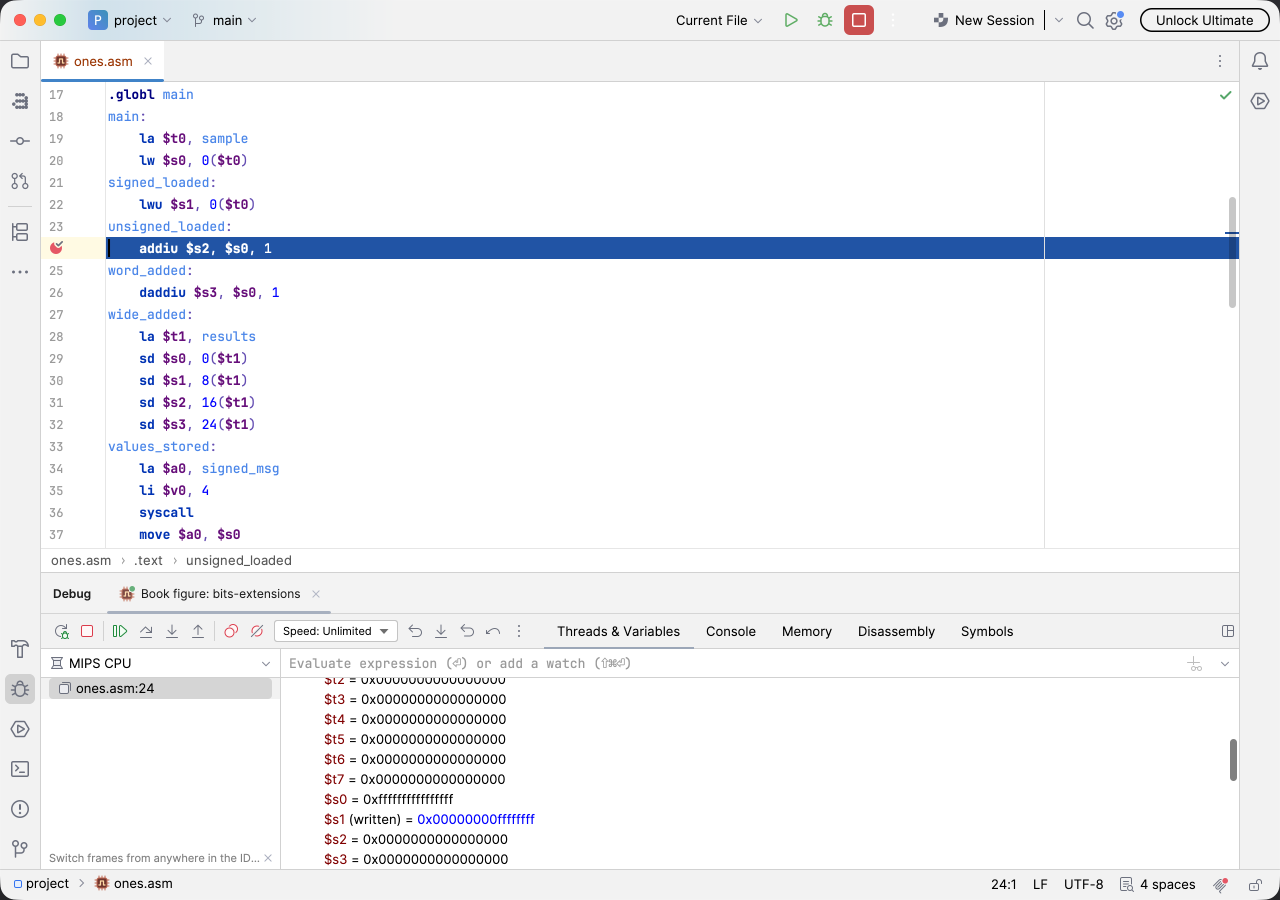
\includegraphics[artifact]{book/captures/004-bit-inspector/f01-extensions/raw.png}}
  \edef\MARSextensionssourceLeft{\the\dimexpr0.036718750\wd0\relax}
  \edef\MARSextensionssourceBottom{\the\dimexpr0.707777778\ht0\relax}
  \edef\MARSextensionssourceRight{\the\dimexpr0.611718750\wd0\relax}
  \edef\MARSextensionssourceTop{\the\dimexpr0.214444444\ht0\relax}
  \edef\MARSextensionssignedLeft{\the\dimexpr0.246093750\wd0\relax}
  \edef\MARSextensionssignedBottom{\the\dimexpr0.097777778\ht0\relax}
  \edef\MARSextensionssignedRight{\the\dimexpr0.639843750\wd0\relax}
  \edef\MARSextensionssignedTop{\the\dimexpr0.873333333\ht0\relax}
  \edef\MARSextensionsunsignedLeft{\the\dimexpr0.246093750\wd0\relax}
  \edef\MARSextensionsunsignedBottom{\the\dimexpr0.075555556\ht0\relax}
  \edef\MARSextensionsunsignedRight{\the\dimexpr0.576562500\wd0\relax}
  \edef\MARSextensionsunsignedTop{\the\dimexpr0.895555556\ht0\relax}
  \begin{tikzpicture}[alt={Three annotated details from one native Debug capture at unsigned_loaded. The next instruction is addiu s2 s0 one. Register s0 contains sixteen hexadecimal f digits; s1 contains eight zero digits followed by eight f digits. Their low 32 bits agree and their upper 32 bits differ.}]
    \node[anchor=north west,inner sep=0,font=\small\bfseries] (source-title) at (6mm,0) {Both loads have completed};
    \node[anchor=north west,inner sep=0] (source) at ([yshift=-1mm]source-title.south west) {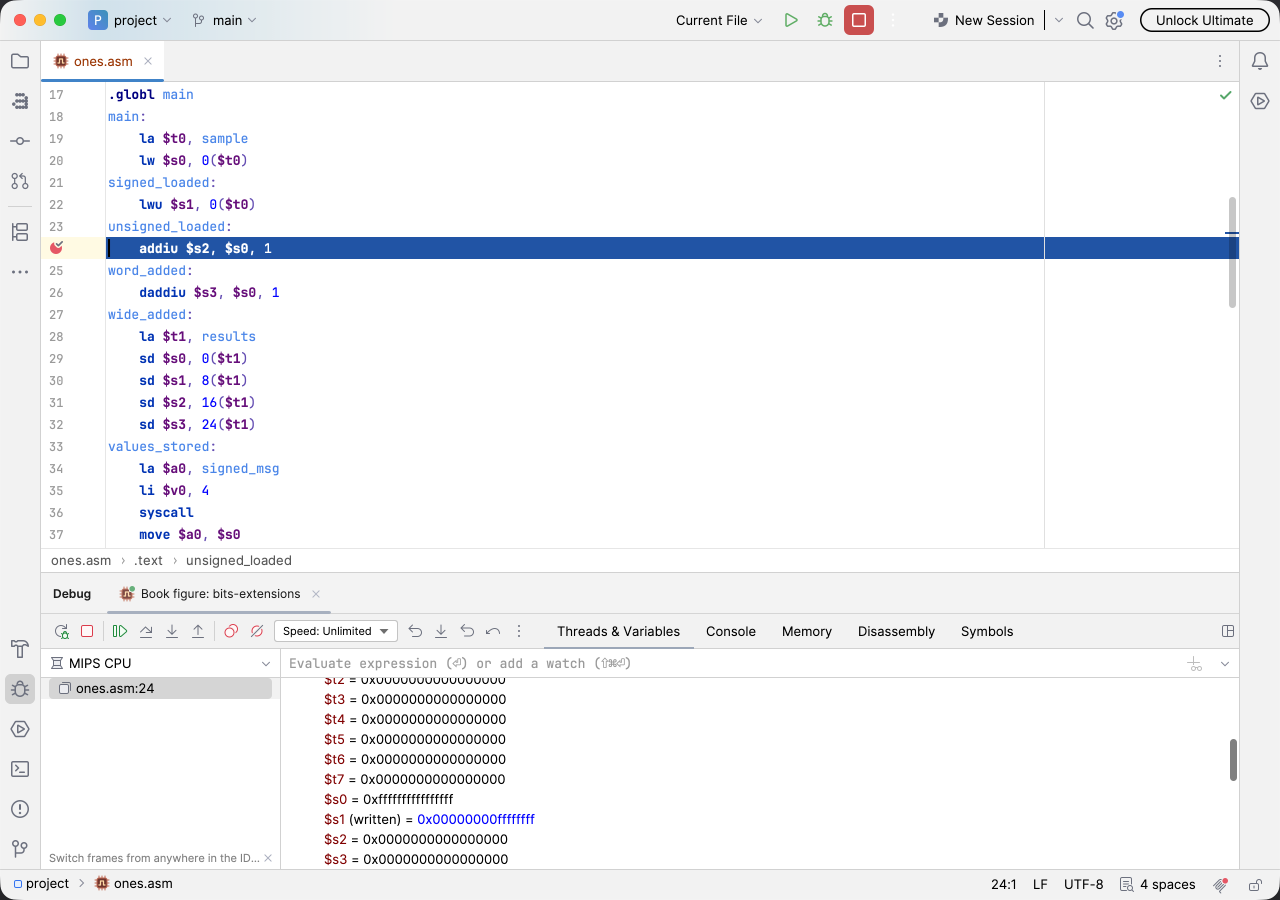
\includegraphics[width=0.7\linewidth,artifact,trim={\MARSextensionssourceLeft{} \MARSextensionssourceBottom{} \MARSextensionssourceRight{} \MARSextensionssourceTop{}},clip]{book/captures/004-bit-inspector/f01-extensions/raw.png}};
    \begin{scope}[shift={(source.south west)},x={($(source.south east)-(source.south west)$)},y={($(source.north west)-(source.south west)$)}]
      \draw[black,line width=0.7pt] (0.135555556,0.057142857) rectangle (0.497777778,0.371428571);
      \node[draw=black,fill=white,circle,inner sep=1.5pt,font=\footnotesize] at ($(0.135555556,0.371428571)+(-3mm,0)$) {1};
    \end{scope}
    \node[anchor=north west,inner sep=0,font=\small\bfseries] (signed-title) at ([yshift=-2mm]source.south west) {The sign-extended word};
    \node[anchor=north west,inner sep=0] (signed) at ([yshift=-1mm]signed-title.south west) {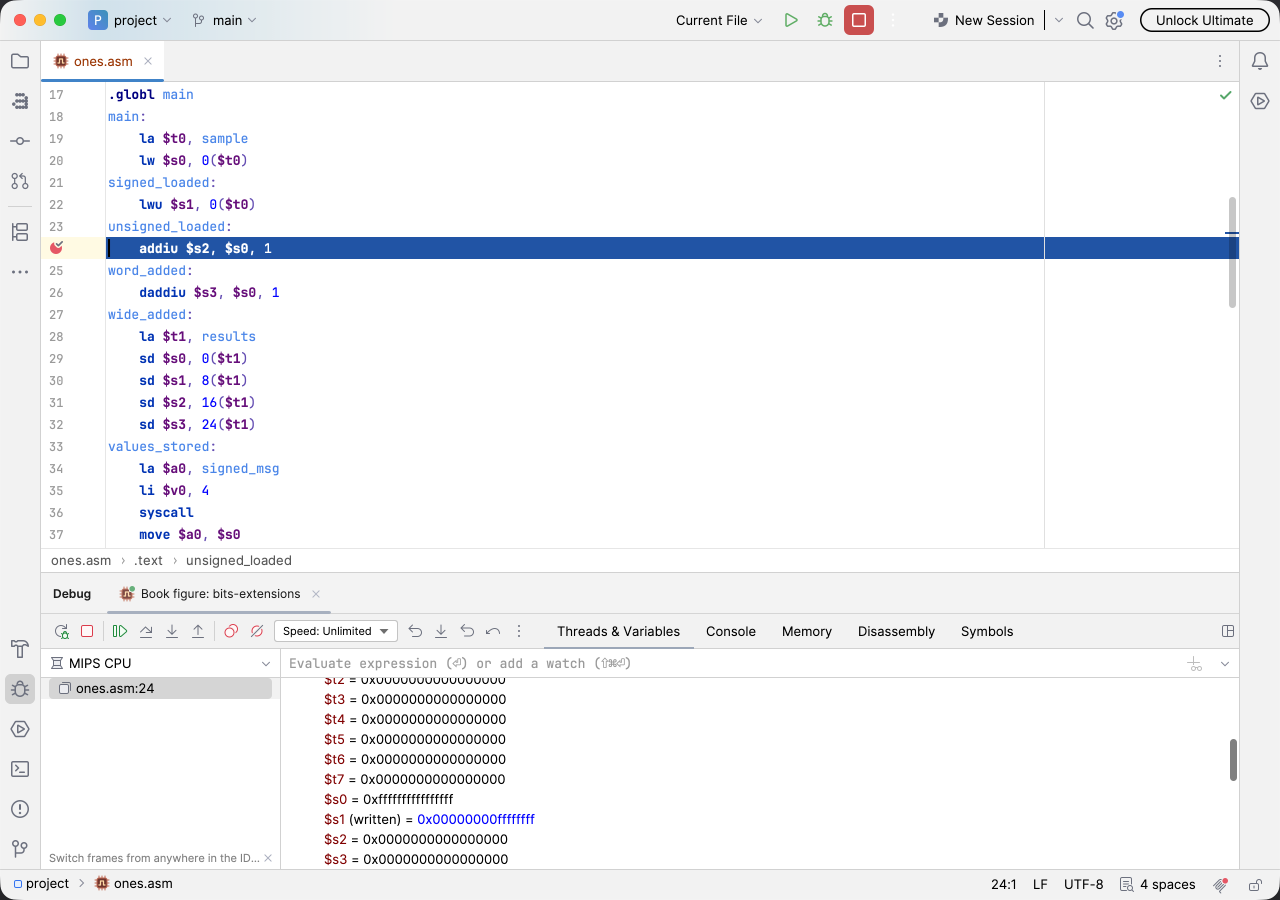
\includegraphics[width=0.53\linewidth,artifact,trim={\MARSextensionssignedLeft{} \MARSextensionssignedBottom{} \MARSextensionssignedRight{} \MARSextensionssignedTop{}},clip]{book/captures/004-bit-inspector/f01-extensions/raw.png}};
    \begin{scope}[shift={(signed.south west)},x={($(signed.south east)-(signed.south west)$)},y={($(signed.north west)-(signed.south west)$)}]
      \draw[black,line width=0.7pt] (0.041095890,0.115384615) rectangle (0.958904110,0.884615385);
      \node[draw=black,fill=white,circle,inner sep=1.5pt,font=\footnotesize] at ($(0.041095890,0.884615385)+(-3mm,0)$) {2};
    \end{scope}
    \node[anchor=north west,inner sep=0,font=\small\bfseries] (unsigned-title) at ([yshift=-2mm]signed.south west) {The zero-extended word};
    \node[anchor=north west,inner sep=0] (unsigned) at ([yshift=-1mm]unsigned-title.south west) {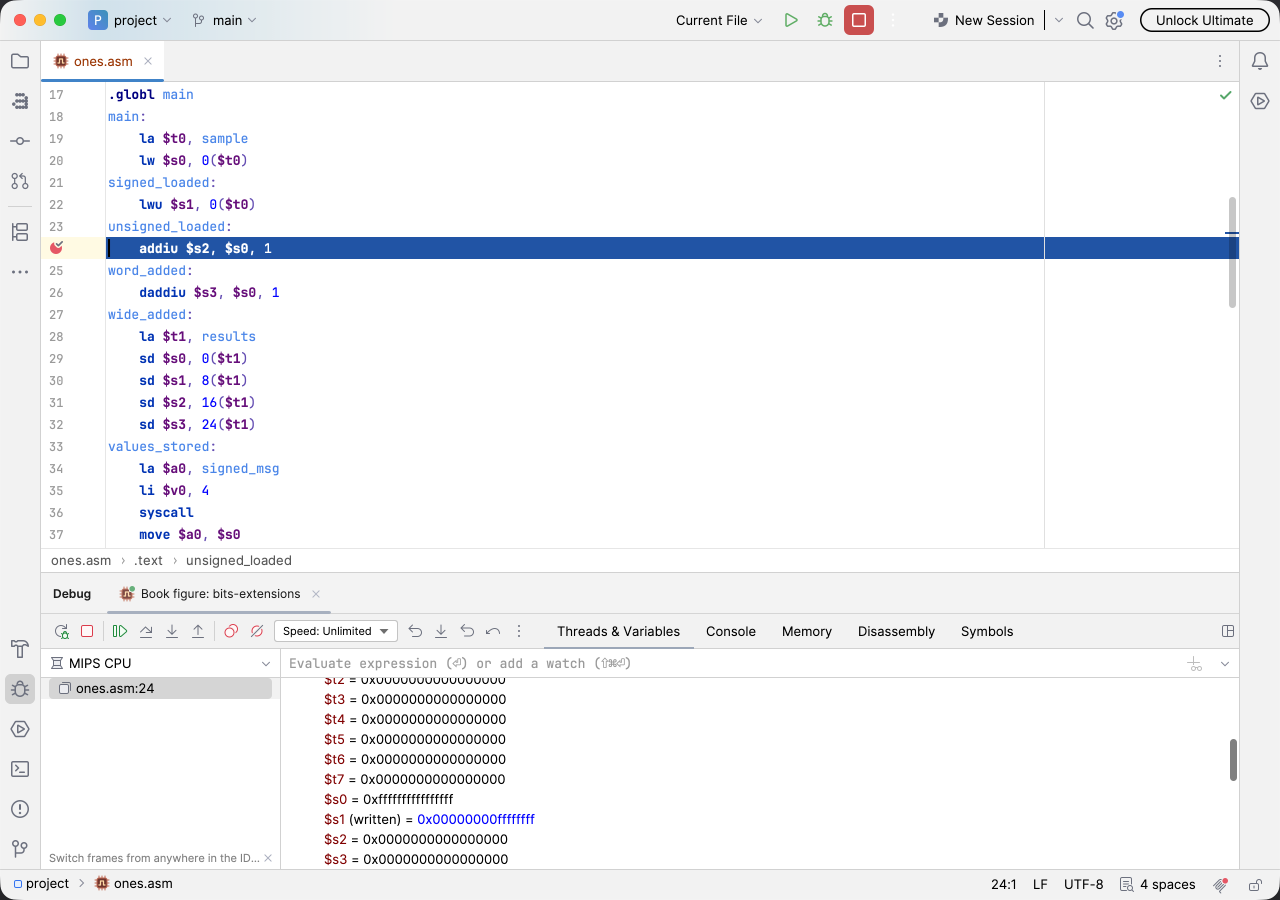
\includegraphics[width=0.53\linewidth,artifact,trim={\MARSextensionsunsignedLeft{} \MARSextensionsunsignedBottom{} \MARSextensionsunsignedRight{} \MARSextensionsunsignedTop{}},clip]{book/captures/004-bit-inspector/f01-extensions/raw.png}};
    \begin{scope}[shift={(unsigned.south west)},x={($(unsigned.south east)-(unsigned.south west)$)},y={($(unsigned.north west)-(unsigned.south west)$)}]
      \draw[black,line width=0.7pt] (0.026431718,0.115384615) rectangle (0.973568282,0.884615385);
      \node[draw=black,fill=white,circle,inner sep=1.5pt,font=\footnotesize] at ($(0.026431718,0.884615385)+(-3mm,0)$) {3};
    \end{scope}
  \end{tikzpicture}
  \par\smallskip
  \begin{minipage}{\linewidth}
    \small
    \begin{enumerate}
      \item The blue line is \texttt{addiu \$s2, \$s0, 1}, before that addition executes. \texttt{lw} has loaded \texttt{\$s0}, and the preceding \texttt{lwu} has loaded \texttt{\$s1} from the same four memory bytes.
      \item \texttt{\$s0}=\texttt{0xffffffffffffffff}. The word has bit 31 set, so \texttt{lw} copies that sign bit through the upper 32 register bits. Interpreted as a signed 64-bit integer, this value is $-1$.
      \item \texttt{\$s1}=\texttt{0x00000000ffffffff}=4294967295. \texttt{lwu} fills the upper half with zero. Both registers have low word \texttt{ffffffff}; inspecting only those eight hexadecimal digits would conceal the extension difference.
    \end{enumerate}
  \end{minipage}
  \caption{After loading the same all-one word with two extension rules. The next instruction has not added one yet.}
  \label{capture:004-bit-inspector-f01-extensions}
\end{figure}
\par
